% Three singular simplices in a space X: a point sigma^0, a path sigma^1, a disk sigma^2.
% Source: book/tex/homology/singular.tex (§ Simplices and boundaries).
\documentclass[border=2mm]{standalone}
\usepackage{tikz}
\usetikzlibrary{arrows.meta}
\definecolor{heavygreen}{rgb}{0,0.5,0}
\begin{document}
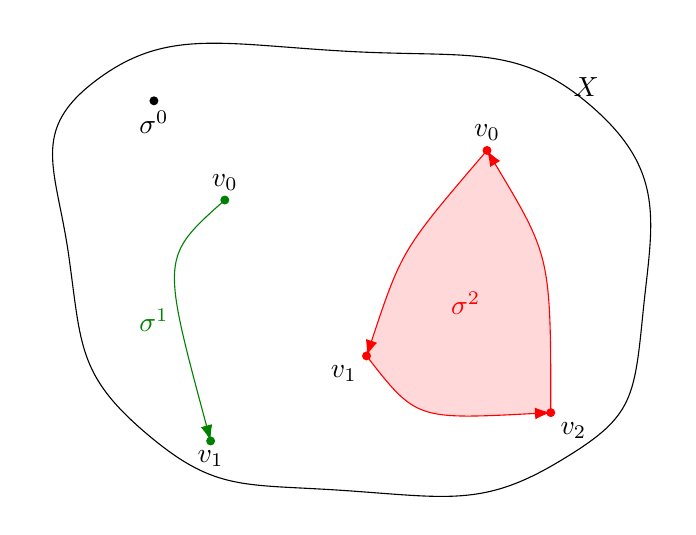
\begin{tikzpicture}[>={Latex[length=2mm]}, scale=0.9]
  % blob X
  \draw plot[smooth cycle, tension=0.9]
    coordinates {(-4.5,2.8) (-1,3.2) (2.5,2.4) (3.2,-0.5) (2,-2.6) (-1,-3) (-3.8,-2.2) (-4.9,0.3)};
  \node at (2.4,2.7) {$X$};
  % sigma^0
  \fill (-3.7,2.5) circle (1.8pt);
  \node[below] at (-3.7,2.5) {$\sigma^0$};
  % sigma^1 (green path)
  \draw[heavygreen, ->] (-2.7,1.1) .. controls (-3.6,0.3) .. (-2.9,-2.3);
  \fill[heavygreen] (-2.7,1.1) circle (1.8pt); \node[above] at (-2.7,1.1) {$v_0$};
  \fill[heavygreen] (-2.9,-2.3) circle (1.8pt); \node[below] at (-2.9,-2.3) {$v_1$};
  \node[heavygreen] at (-3.7,-0.6) {$\sigma^1$};
  % sigma^2 (red filled curved triangle)
  \coordinate (B0) at (1,1.8);
  \coordinate (B1) at (-0.7,-1.1);
  \coordinate (B2) at (1.9,-1.9);
  \fill[red!15]
    (B0) .. controls (-0.2,0.4) .. (B1)
    .. controls (0,-2) .. (B2)
    .. controls (1.9,0.3) .. (B0);
  \draw[red, ->] (B0) .. controls (-0.2,0.4) .. (B1);
  \draw[red, ->] (B1) .. controls (0,-2) .. (B2);
  \draw[red, ->] (B2) .. controls (1.9,0.3) .. (B0);
  \fill[red] (B0) circle (1.8pt); \node[above] at (B0) {$v_0$};
  \fill[red] (B1) circle (1.8pt); \node[below left] at (B1) {$v_1$};
  \fill[red] (B2) circle (1.8pt); \node[below right] at (B2) {$v_2$};
  \node[red] at (0.7,-0.35) {$\sigma^2$};
\end{tikzpicture}
\end{document}
